% ==========================================================
% Docent: AI-Driven Presentation Generation and Delivery
% from Multimodal Sources
%
% arXiv preprint — cs.HC
% Draft 2 — March 2026
% ==========================================================
\documentclass[11pt,a4paper]{article}

% ── Geometry & Layout ─────────────────────────────────────
\usepackage[margin=1in]{geometry}
\usepackage{setspace}
\onehalfspacing

% ── Fonts & Encoding ──────────────────────────────────────
\usepackage[T1]{fontenc}
\usepackage[utf8]{inputenc}
\usepackage{lmodern}
\usepackage{microtype}

% ── Math & Symbols ────────────────────────────────────────
\usepackage{amsmath,amssymb}

% ── Graphics & Figures ────────────────────────────────────
\usepackage{graphicx}
\usepackage{tikz}
\usetikzlibrary{arrows.meta,positioning,shapes.geometric,fit,backgrounds}
\usepackage{float}
\usepackage{subcaption}

% ── Tables ────────────────────────────────────────────────
\usepackage{booktabs}
\usepackage{multirow}
\usepackage{array}
\usepackage{tabularx}
\usepackage{makecell}
\usepackage{pdflscape}

% ── Colors & Hyperlinks ──────────────────────────────────
\usepackage[dvipsnames]{xcolor}
\usepackage[colorlinks=true,linkcolor=MidnightBlue,citecolor=MidnightBlue,urlcolor=MidnightBlue]{hyperref}

% ── Bibliography ──────────────────────────────────────────
\usepackage[sort&compress,numbers]{natbib}
\bibliographystyle{unsrtnat}

% ── Listings (code snippets) ──────────────────────────────
\usepackage{listings}
\lstdefinelanguage{json}{
  basicstyle=\ttfamily\small,
  string=[s]{"}{"},
  stringstyle=\color{Emerald!80!black},
  comment=[l]{//},
  morestring=[b]',
  literate=
    *{:}{{{\color{BurntOrange}{:}}}}{1}
     {,}{{{\color{BurntOrange}{,}}}}{1}
     {\{}{{{\color{gray}{\{}}}}{1}
     {\}}{{{\color{gray}{\}}}}}{1}
     {[}{{{\color{gray}{[}}}}{1}
     {]}{{{\color{gray}{]}}}}{1}
}
\lstset{
  basicstyle=\ttfamily\small,
  breaklines=true,
  frame=single,
  backgroundcolor=\color{gray!8},
  keywordstyle=\color{MidnightBlue}\bfseries,
  commentstyle=\color{OliveGreen},
  stringstyle=\color{BrickRed},
}

% ── Misc ──────────────────────────────────────────────────
\usepackage{enumitem}
\usepackage{url}
\usepackage{xspace}

% ── Custom commands ───────────────────────────────────────
\newcommand{\system}{\textsc{Docent}\xspace}
\newcommand{\sage}{\textsc{Sage}\xspace}

% ══════════════════════════════════════════════════════════
% FRONT MATTER
% ══════════════════════════════════════════════════════════
\title{%
  \textbf{Docent: Human--AI Symbiotic Loop\\
  from Research to Understanding}%
}

\author{%
  Ilknur Icke\\
  Symbiont-AI Cognitive Labs\\
  \texttt{https://github.com/symbiont-ai/docent}
}

\date{March 2026}

\begin{document}
\maketitle

% ──────────────────────────────────────────────────────────
% ABSTRACT
% ──────────────────────────────────────────────────────────
\begin{abstract}
Document understanding, research curation, and educational delivery have largely been studied as separate problems: one focuses on extracting knowledge from papers, another on curating knowledge about topics from scattered sources, and a third on communicating it effectively to learners.
We argue that connecting these ends creates a \emph{symbiotic loop}---an iterative cycle of bidirectional questioning between human and AI.
The human questions the AI, driven by curiosity and debate; the AI questions the human, assessing comprehension and surfacing knowledge gaps.
Through this exchange, the pair converges on understanding more effectively than either could alone.
Drawing on Licklider's vision of human--computer symbiosis~\citep{licklider1960symbiosis} and closed-loop perspectives on symbiotic interaction~\citep{fairclough2015closedloop}, we present \system, an open-source, browser-based platform that instantiates this loop through an AI persona called \sage.
Given a research paper, technical report, or free-form topic, \sage engages the user in a conversational workflow spanning the full research-to-learning arc: it curates knowledge through vision-based document analysis and web-grounded research with deep reasoning, synthesizes content into structured slide presentations with custom SVG diagrams and extracted figures, delivers narrated lectures through a dual text-to-speech pipeline, and supports post-presentation Q\&A for comprehension reinforcement.

Critically, \system treats this pipeline not as a batch process but as an interactive dialogue.
Users shape presentations through conversational refinement, observe slides streaming incrementally as they are generated, and transition seamlessly from content delivery to knowledge assessment---all within a single conversational interface.
Two governance concerns are asymmetrically assigned: hallucination prevention is the AI's structural responsibility---ensuring content fidelity before delivery, as a responsible teacher would---while assessment of understanding is the AI's pedagogical role, verifying that each cycle produces genuine learning.
We describe the system architecture, methodology, and a detailed evaluation plan.
\system is released under the MIT license.
\end{abstract}

\noindent\textbf{Keywords:} symbiotic loop, document understanding, research curation, educational AI, human--AI symbiosis, presentation generation, conversational AI, large language models, interactive learning

% ══════════════════════════════════════════════════════════
\newpage
\section{Introduction}
\label{sec:intro}
% ══════════════════════════════════════════════════════════

Research papers and technical documents are the primary vehicles for scientific knowledge, yet they are notoriously difficult to absorb---dense prose, domain-specific notation, and complex figures create barriers for students, interdisciplinary researchers, and practitioners seeking to learn from unfamiliar fields.
Even when the goal is to learn about a \emph{topic} rather than a specific paper, the challenge persists: relevant knowledge is scattered across multiple sources, rapidly evolving, and difficult to curate without domain expertise.
Presentations and lectures have long served as the bridge between written knowledge and human comprehension, but creating an effective presentation---whether from a single paper or from research across a field---remains labor-intensive, requiring source curation, content synthesis, visual design, figure selection, diagram creation, and narration scripting.

\begin{figure}[t]
\centering
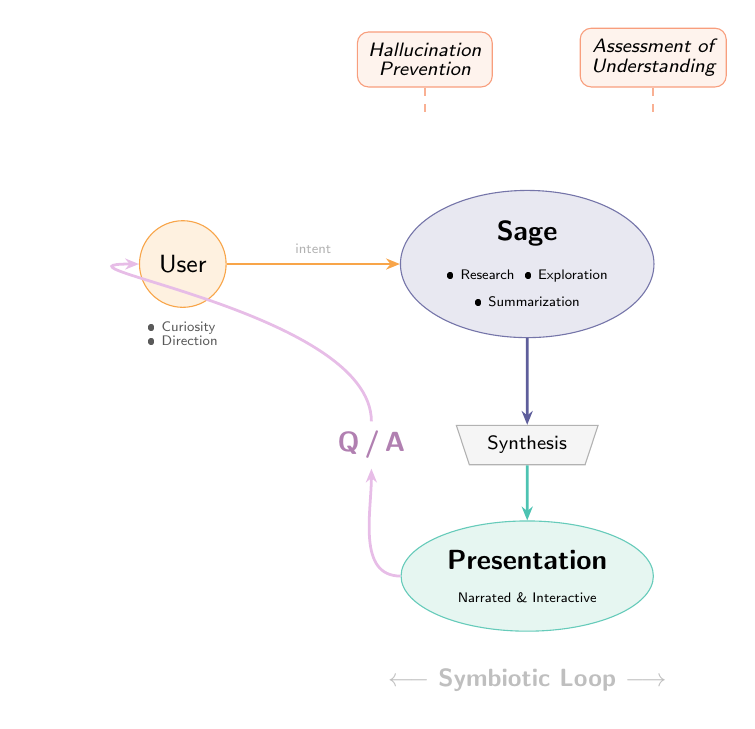
\begin{tikzpicture}[
    node distance=0.9cm,
    >=Stealth,
    agent/.style={
        ellipse, draw=#1!60, fill=#1!10,
        minimum width=2.6cm, minimum height=1.4cm,
        align=center, font=\sffamily\small
    },
    agent/.default=MidnightBlue,
    usernode/.style={
        circle, draw=BurntOrange!70, fill=BurntOrange!10,
        minimum size=1.1cm, align=center, font=\sffamily\small
    },
    funnel/.style={
        trapezium, trapezium angle=70, trapezium stretches body,
        draw=gray!60, fill=gray!8,
        minimum width=1.8cm, minimum height=0.5cm,
        align=center, font=\sffamily\tiny,
        shape border rotate=180
    },
    concern/.style={
        draw=RedOrange!50, fill=RedOrange!6, rounded corners=4pt,
        align=center, font=\sffamily\scriptsize\itshape,
        inner sep=4pt
    },
    loopflow/.style={
        -{Stealth[length=5pt, width=4pt]}, thick, color=#1!70,
        line width=1pt
    },
    loopflow/.default=MidnightBlue,
    blabel/.style={
        font=\sffamily\tiny, text=gray!70!black, align=left
    },
]

% ── User ──
\node[usernode] (user) {User};
\node[blabel, below=0.05cm of user, anchor=north] {
    \textbullet\ Curiosity\\[-1pt]
    \textbullet\ Direction
};

% ── Sage ──
\node[agent=MidnightBlue, right=2.2cm of user, minimum height=1.7cm] (sage) {
    {\normalsize\bfseries Sage}\\[3pt]
    {\tiny\textbullet\ Research~~\textbullet\ Exploration}\\[-1pt]
    {\tiny\textbullet\ Summarization}
};

% ── Funnel ──
\node[funnel, below=1.1cm of sage] (funnel) {\scriptsize Synthesis};

% ── Presentation ──
\node[agent=Emerald, below=0.7cm of funnel] (pres) {
    {\normalsize\bfseries Presentation}\\[1pt]
    {\tiny Narrated \& Interactive}
};

% ── Q/A label ──
\node[font=\sffamily\normalsize\bfseries, text=Plum!80!black,
      left=0.6cm of funnel] (qa) {Q\,/\,A};

% ── Flow arrows ──
\draw[loopflow=BurntOrange] (user) -- node[above, font=\sffamily\tiny, text=gray!60] {intent} (sage);
\draw[loopflow=MidnightBlue] (sage) -- (funnel);
\draw[loopflow=Emerald] (funnel) -- (pres);
\draw[loopflow=Plum] (pres.west) to[out=180, in=-90] (qa.south);
\draw[loopflow=Plum] (qa.north) to[out=90, in=180] (user.west);

% ── Overarching concerns ──
\node[concern, above=1.3cm of sage, xshift=-1.3cm] (halluc) {
    Hallucination\\[-1pt]Prevention
};
\node[concern, above=1.3cm of sage, xshift=1.6cm] (assess) {
    Assessment of\\[-1pt]Understanding
};

\draw[dashed, RedOrange!40, thick] (halluc.south) -- ++(0, -0.4);
\draw[dashed, RedOrange!40, thick] (assess.south) -- ++(0, -0.4);

% ── Symbiotic Loop label ──
\node[below=0.35cm of pres, font=\sffamily\small\bfseries, text=gray!50] {
    $\longleftarrow$~Symbiotic Loop~$\longrightarrow$
};

\end{tikzpicture}
\caption{The Symbiotic Loop: \system's conceptual framework. The user provides curiosity and direction; \sage researches, explores, and synthesizes content into a narrated presentation. In the Q\&A phase, the human asks curiosity-driven questions or offers corrections from their own expertise, while \sage probes the user's understanding. Two governance concerns are asymmetrically assigned: hallucination prevention is the AI's structural responsibility (ensuring content fidelity before delivery), while assessment of understanding is the AI's pedagogical role (verifying that learning has occurred).}
\label{fig:symbiotic-loop}
\end{figure}

These three challenges---\emph{document understanding}, \emph{research curation}, and \emph{educational delivery}---have largely been addressed independently.
Document AI systems extract text, figures, and structure from PDFs but do not communicate what they find.
Research tools like Perplexity and SciSpace curate knowledge from web and academic sources but do not synthesize it into structured educational content.
Presentation generation systems produce slides from text inputs but lack deep comprehension or research capabilities.
Educational tools like NotebookLM generate slide decks and audio summaries from documents but treat these as one-shot outputs without conversational refinement, iterative editing, or bidirectional assessment.
We argue that connecting these capabilities into a single conversational pipeline---from research and comprehension through communication to assessment---creates what we term a \emph{symbiotic loop} (Figure~\ref{fig:symbiotic-loop}): an iterative cycle of \textbf{bidirectional questioning} between human and AI.
The human questions the AI---driven by curiosity, proposing corrections, or debating interpretations from their own perspective.
The AI questions the human---generating comprehension challenges, identifying knowledge gaps, and adapting subsequent iterations to address them.
Crucially, these two directions carry distinct responsibilities.
Hallucination prevention is the \emph{AI's} structural obligation: like a responsible teacher, \sage must ensure that what it presents is valid and supported by verifiable sources \emph{before} presenting it---the loop does not depend on the human to catch errors, though users may naturally challenge or correct content from their own expertise.
Assessment of understanding is the AI's \emph{pedagogical} role: probing whether genuine learning has occurred.
Neither direction alone is sufficient: the human can synthesize research into presentations, but the ever-growing volume of scientific literature makes this increasingly impractical without AI assistance.
The AI, meanwhile, cannot know what the human does not yet understand.
Through iterative exchange, they converge on understanding that neither could reach as effectively alone.


This concept draws on Licklider's foundational vision of human--computer symbiosis~\citep{licklider1960symbiosis}, in which humans set goals and formulate hypotheses while machines handle routinizable information processing, and on Fairclough's closed-loop perspective on symbiotic interaction~\citep{fairclough2015closedloop}, which characterizes effective human--computer partnerships as bidirectional feedback cycles.
Licklider's central question---can the human--machine partnership ``perform intellectual operations much more effectively than man alone can perform them''---motivates our design.
Where prior work has applied these ideas to physiological computing and adaptive interfaces, we instantiate the symbiotic loop specifically for educational AI: the human brings curiosity, judgment, and the ability to recognize genuine understanding, while the AI brings research capacity, synthesis at scale, and the ability to systematically probe for comprehension gaps.
The idea of AI agents as learning partners is itself well-established: early work on agent-based learning partners used simulation and human behavioral data to train agents that emulate learner patterns in adaptive educational assessments~\citep{sklar2009simulation}.
\system extends this vision with modern LLMs---rather than emulating learner behavior, \sage acts as a knowledgeable partner that researches, teaches, and assesses, closing the bidirectional loop that earlier agent-based systems left open.
The emergence of large language models with multimodal capabilities~\citep{openai2023gpt4, anthropic2024claude, team2023gemini} makes this integration feasible: a single model can now read a PDF, search the web for current sources, synthesize findings, generate structured slides, and engage in follow-up dialogue---in both directions.
Moreover, the choice of narrated, interactive presentations as the delivery medium is not incidental.
Formal education has always been built around a teacher who explains, shows, and questions---multimodal interaction is how humans are wired to learn~\citep{mayer2009multimedia}.
\sage replicates this modality: it narrates while displaying visual content, adapts explanations through dialogue, and assesses comprehension through questioning, mirroring the teacher--student dynamic that has anchored human learning for millennia.

The ultimate promise of the symbiotic loop extends beyond comprehension of existing knowledge.
When human and AI engage in sustained iterative exchange---each questioning the other, each contributing what the other lacks---the collaboration can generate \emph{novel ideas and understanding} that neither party would have reached alone.
This paper and the system it describes are themselves products of such a loop: the conceptual framework, technical design, and research contributions emerged through iterative human--AI dialogue in which direction, judgment, and domain expertise combined with research synthesis, implementation capacity, and systematic exploration.
\system's current instantiation targets the comprehension end of this spectrum, but the symbiotic loop framework points toward a deeper goal: \emph{collaborative discovery}, in which the iterative cycle produces not just understanding of what is known, but insight into what is not yet known.

We present \system, an open-source, browser-based platform that instantiates the symbiotic loop through an AI persona called \sage.
Given a research paper, technical report, or free-form topic, \sage engages users in a conversational workflow spanning the full research-to-learning arc:

\begin{enumerate}[leftmargin=*,nosep]
    \item \textbf{Research \& Comprehension.} \sage operates in two modes: given an uploaded document, it reads and analyzes multimodal content via vision-based PDF analysis; given a free-form topic, it curates knowledge through web search grounded in live sources. An optional deep thinking mode allocates extended reasoning to produce more thorough content plans for complex subjects.
    \item \textbf{Synthesis.} It generates structured slide presentations with custom SVG diagrams, extracted PDF figures or web-sourced references, and configurable layouts, streaming slides incrementally as they are produced.
    \item \textbf{Delivery.} A dual text-to-speech pipeline narrates the presentation with cross-slide prefetch buffering, transforming static slides into a narrated lecture experience.
    \item \textbf{Interaction.} Users refine presentations through conversational dialogue, requesting modifications, additions, or restructuring at any point.
    \item \textbf{Assessment.} The questioning reverses direction: \sage generates comprehension questions to probe the user's understanding, while users ask curiosity-driven questions, propose corrections, or debate interpretations from their own expertise. This bidirectional Q\&A closes the loop---the AI identifies knowledge gaps that inform the next iteration of the cycle.
\end{enumerate}

Critically, \system treats this entire pipeline as an interactive dialogue rather than a batch process.
Unlike prior systems that produce slides as a one-shot output, \system enables iterative refinement through conversation, progressive rendering through streaming generation, and seamless transition from delivery to assessment---all within a single interface.

Our contributions span both the document understanding and educational delivery sides of this bridge:

\begin{itemize}[leftmargin=*,nosep]
    \item A \textbf{conversational research-to-learning pipeline} that unifies document comprehension, web-grounded research curation, presentation synthesis, narrated delivery, and post-generation Q\&A under a single AI persona, connecting capabilities that have previously been studied in isolation.
    \item A \textbf{vision-guided PDF figure extraction} mechanism that uses LLM-predicted normalized coordinates to crop specific figures, tables, and diagrams from source documents, with automatic whitespace trimming.
    \item An \textbf{SVG diagram synthesis} methodology that instructs the LLM to produce inline vector diagrams across ten distinct diagram types under strict theme and quality constraints.
    \item A \textbf{streaming slide generation} architecture that renders slides incrementally as the LLM produces them, reducing perceived latency and enabling early user feedback.
    \item A \textbf{dual TTS narration system} combining browser-native Web Speech API with optional neural TTS via Google Gemini, featuring cross-slide prefetch buffering for seamless lecture delivery.
    \item A complete, open-source \textbf{implementation} as a browser-based web application with multi-model support, multilingual generation, and multi-format export, released under the MIT license.
\end{itemize}


% ══════════════════════════════════════════════════════════
\section{Related Work}
\label{sec:related}
% ══════════════════════════════════════════════════════════

\subsection{Commercial AI Presentation Tools}

Several commercial tools have explored AI-assisted presentation creation.
\textbf{Gamma}\footnote{\url{https://gamma.app}} generates presentations from text prompts using templates and stock imagery, and has emerged as the leading web-native AI presentation tool with tens of millions of users and a profitable business model.
\textbf{Beautiful.ai}\footnote{\url{https://www.beautiful.ai}} applies design rules to automatically adjust slide layouts, offering a structured JSON schema for partial programmatic control.
\textbf{SlidesAI}\footnote{\url{https://www.slidesai.io}} integrates with Google Slides to convert text into slides.
\textbf{Canva}\footnote{\url{https://www.canva.com}} is the dominant general-purpose design platform with over 240 million monthly users; its ``Magic Design'' feature generates AI presentations from prompts, supported by an extensive template and asset library.
These tools primarily focus on template-driven layout and stock image placement.
In contrast, \system generates \emph{custom} SVG diagrams, extracts figures from user-uploaded documents, and supports iterative conversational refinement and post-generation Q\&A---producing information-dense visual content rather than relying on generic imagery.
Table~\ref{tab:comparison} provides a detailed feature comparison across commercial and academic systems.

\subsection{Academic Presentation Generation Systems}

Academic work on automated slide generation has evolved through three overlapping phases: task-specific trained models, prompting-based pipelines, and hybrid approaches.

\paragraph{Task-specific models.}
Early systems trained dedicated models on paired document--slide datasets.
\textbf{Doc2PPT}~\citep{fu2022doc2ppt} formalized the document-to-slides task and proposed a hierarchical sequence-to-sequence model with paraphrasing and layout prediction modules, releasing a 6K-pair dataset drawn from CVPR, ACL, and ICML proceedings.
Doc2PPT established the paradigm of treating slide generation as structured summarization---an approach followed by subsequent work but limited by the need for large paired training corpora.

\paragraph{Prompting-based pipelines.}
The emergence of capable foundation models shifted the field toward prompting-based pipelines that orchestrate commercial LLMs without training new models.
These systems differ primarily in their \emph{input requirements} and \emph{pipeline design}, as none trains task-specific parameters.

\textbf{PPTAgent}~\citep{zheng2025pptagent} proposes a two-stage edit-based approach: it first analyzes \emph{reference presentations} to extract functional slide types and content schemas, then generates new slides through LLM-produced code actions that modify selected reference slides.
PPTAgent also introduces PPTEval, a multidimensional evaluation framework assessing Content, Design, and Coherence.
However, PPTAgent requires existing reference presentations as input---it cannot generate slides from scratch.

\textbf{SlideTailor}~\citep{zeng2026slidetailor} addresses the subjectivity of presentation design by conditioning generation on implicit user preferences.
Given a paper--slides \emph{example pair} and a \texttt{.pptx} visual template, SlideTailor distills preferences across content and aesthetics, then applies a ``chain-of-speech'' mechanism that plans oral narration before deriving slide content.
Built on PPTAgent's codebase, it introduces the PSP benchmark with interpretable metrics.
Like PPTAgent, SlideTailor requires pre-existing presentation artifacts as input.

\textbf{PresentAgent}~\citep{wu2025presentagent} extends the scope to full presentation \emph{video} generation, routing among six LLM backends (GPT-4o, Gemini, Claude, Qwen-VL) with dynamic selection, using a VLM critic for visual quality feedback and MegaTTS3 for speech synthesis.
It targets offline video production from documents rather than interactive presentation.

\textbf{SlideBot}~\citep{xie2026slidebot} is a multi-agent framework grounded in Cognitive Load Theory and the Cognitive Theory of Multimedia Learning.
A Moderator--Retriever agent pair generates search keywords and retrieves academic papers from arXiv, a Code Generator produces LaTeX Beamer slides, and an Enhancer inserts figures.
SlideBot is the only academic system that generates presentations from \emph{topics} (via retrieval) rather than requiring pre-existing documents, paralleling \system's topic-based generation mode.

\textbf{SlideGen}~\citep{liang2025slidegen} orchestrates six vision-language agents (Outliner, Mapper, Formulizer, Speaker, Arranger, Refiner) in a visual-in-the-loop pipeline, using VLM feedback to assess layout quality during generation.
It introduces a Geometry-Aware Density metric for evaluating visual aesthetics and claims state-of-the-art results across multiple benchmarks.

\paragraph{Hybrid: training meets prompting.}
\textbf{AutoPresent}~\citep{ge2025autopresent} is the only system in this landscape that trains a dedicated model: an 8B LLaMA model fine-tuned on 7K instruction--code pairs for slide generation via \texttt{python-pptx} code generation.
It introduces SlidesBench, the first benchmark for slide generation with reference-based and reference-free evaluation.
AutoPresent achieves results comparable to GPT-4o despite being 8B parameters, but generates individual slides from explicit instructions rather than complete presentations from documents.

\paragraph{Positioning of \system.}
All systems above---whether trained or prompted---share a common limitation: they treat presentation generation as a \emph{batch} process.
The user provides inputs, the system produces slides, and the interaction ends.
None supports conversational refinement during generation, iterative dialogue-based editing after generation, or post-presentation Q\&A for comprehension.
\system is, to our knowledge, the first system that frames presentation generation as a \emph{conversational} process, supporting two co-equal input modes---topic-based generation with web-grounded research curation, and document-based generation with vision analysis---without requiring reference slides, example pairs, or templates, while enabling deep thinking for complex subjects, streaming slide generation (slides render incrementally as the LLM produces them), real-time narration, and post-generation learning through its \sage agent.
Table~\ref{tab:academic} summarizes the input requirements, approaches, and interaction paradigms across all academic systems.

\subsection{Open-Source Presentation Tools}

\textbf{Presenton}~\citep{presenton2025} is an open-source AI presentation generator (4,100+ GitHub stars) that runs locally as an Electron desktop application or Docker container.
It supports multiple LLM providers (OpenAI, Gemini, Ollama) and generates PPTX/PDF exports with stock imagery from Pexels, Pixabay, and DALL-E~3.
Presenton focuses on template-based generation with tone and verbosity controls, and offers an API for programmatic use.
\system differs in several respects: it operates entirely in the browser with zero installation, supports both document-based and web-grounded topic-based generation with deep thinking, generates custom SVG diagrams rather than sourcing stock images, extracts and crops figures directly from uploaded PDFs, provides live TTS narration with dual engine support, and maintains a conversational interface for iterative refinement and post-generation Q\&A.

\subsection{Educational and Research AI Tools}
\label{sec:related-eduresearch}

A growing class of AI tools targets document understanding, knowledge synthesis, and educational content creation, overlapping with \system's capabilities along the research-to-presentation pipeline.

\textbf{NotebookLM}\footnote{\url{https://notebooklm.google.com}} (Google) is a document-grounded AI research assistant powered by Gemini.
Users upload PDFs, Google Docs, web URLs, and other sources into notebooks, then interact through conversational Q\&A with inline clickable citations to source passages.
NotebookLM's Studio panel generates multiple output formats from the same sources: Audio Overviews (podcast-style discussions between two AI hosts with an interactive ``Join'' mode), Video Overviews (narrated slide-style videos with AI-generated visuals and diagrams), slide decks and infographics (powered by Google's Nano Banana Pro image generation model), mind maps, reports, quizzes, and flashcards.
Deep Research mode performs agentic web browsing for multi-source reports.
NotebookLM is arguably the closest system to \system in scope, but key architectural differences remain: its slides are image-based rather than structured (not editable PPTX), figure extraction from source PDFs is limited, slide decks cannot be incrementally edited through conversation---users must regenerate entirely---and there is no bidirectional assessment loop in which the AI probes the user's comprehension.
\system addresses these gaps with editable structured slides, vision-based figure extraction, custom SVG diagrams, iterative conversational refinement, and the symbiotic loop's bidirectional questioning.

\textbf{Perplexity}\footnote{\url{https://www.perplexity.ai}} is a research-focused AI engine combining real-time web search with multi-model inference (GPT, Claude, Gemini).
Its Deep Research mode performs multi-step autonomous web browsing, and every response includes numbered citations to source web pages.
Perplexity can generate downloadable PPTX presentations via its ``Create files and apps'' feature and supports an Academic Filter for scholarly source retrieval.
However, Perplexity is a general-purpose research tool without education-specific features such as quiz generation, pedagogical grounding, or post-presentation assessment.

\textbf{SciSpace}\footnote{\url{https://scispace.com}} (formerly Typeset.io) provides AI-powered research paper analysis with a focus on academic literature.
Its Copilot feature enables conversational Q\&A with PDF papers, and users can ``snip'' equations, tables, and figures directly from documents for AI-generated explanations---a capability paralleling \system's PDF figure extraction.
SciSpace indexes over 270 million scientific articles and supports 75+ languages.
However, SciSpace cannot generate presentations, positioning it as a complementary research tool rather than a direct competitor.

Several open-source projects have emerged as self-hosted alternatives to NotebookLM, prioritizing data privacy and model flexibility.
\textbf{Open Notebook}\footnote{\url{https://github.com/lfnovo/open-notebook}}~\citep{opennotebook2025} is the most prominent, with over 4,100 GitHub stars and an MIT license.
Built on Python, FastAPI, and Next.js, it supports 16+ AI providers (including local models via Ollama), offers multi-speaker podcast generation with customizable episode profiles, document Q\&A with citations, and full-text and vector search across notebooks.
\textbf{SurfSense}\footnote{\url{https://github.com/MODSetter/SurfSense}}~\citep{surfsense2025} (12,600+ stars) takes a different approach as a self-hosted RAG-based research agent that integrates with external services (Slack, Notion, Jira, GitHub, Google Drive) to build a unified searchable knowledge base, with a browser extension for capturing web content.
Both tools replicate NotebookLM's core document Q\&A and podcast capabilities in a privacy-preserving, model-agnostic form, but neither generates structured slide presentations, provides narrated delivery, or supports post-presentation assessment---the capabilities that define \system's symbiotic loop.

Table~\ref{tab:comparison-edu} compares \system against these educational and research tools, highlighting how \system uniquely integrates presentation generation with document analysis, web research, and post-generation assessment in a single conversational interface.

\subsection{Large Language Models and Structured Generation}

The capacity of LLMs to generate structured outputs---JSON, code, markup---has been extensively studied~\citep{brown2020language, chen2021evaluating, wei2022chain}.
Recent work on constrained decoding~\citep{willard2023guided} ensures that LLM outputs conform to specified schemas.
Prompt engineering techniques~\citep{reynolds2021prompt} have proven effective at guiding LLMs to produce outputs in particular formats.
\system leverages these capabilities through detailed system prompts that define the JSON slide schema, SVG generation constraints, and layout selection heuristics.

\subsection{Multimodal Document Understanding}

Vision-language models have demonstrated strong performance on document understanding tasks~\citep{liu2023visual, wang2024docllm, li2024multimodal}.
These models can interpret the visual layout of documents, read text from images, and identify structural elements such as figures, tables, and headings.
\system exploits these capabilities by rendering PDF pages as images and including them in the LLM's vision context, enabling the model to identify figure locations and predict crop coordinates without relying on heuristic PDF parsing.

\subsection{Automated Information Visualization}

The field of automated visualization encompasses grammar-based approaches such as Vega-Lite~\citep{satyanarayan2017vegalite} and taxonomic frameworks~\citep{shneiderman1996eyes, heer2010tour}.
Multimedia learning theory~\citep{mayer2009multimedia} and information design principles~\citep{tufte2001visual} emphasize that effective visual communication requires matching diagram types to content semantics.
\system operationalizes this principle by providing the LLM with a taxonomy of ten diagram types---flowcharts, comparison tables, timelines, layered architectures, Venn diagrams, network graphs, bar charts, annotated schematics, matrices, and cycle diagrams---and instructing it to select the most appropriate type for each slide's content.


% ══════════════════════════════════════════════════════════

% ══════════════════════════════════════════════════════════
\section{Approach}
\label{sec:approach}
% ══════════════════════════════════════════════════════════

\system instantiates the symbiotic loop (Figure~\ref{fig:symbiotic-loop}) as a five-stage conversational pipeline.
Unlike batch-mode systems that treat presentation generation as a one-shot process, \system frames the interaction as an iterative cycle in the spirit of Licklider's human--computer symbiosis~\citep{licklider1960symbiosis}: the user provides curiosity and direction, \sage researches and synthesizes, a narrated presentation is delivered, and post-presentation Q\&A generates new questions that feed back into the loop.
Each iteration deepens understanding, governed by two asymmetric responsibilities: \emph{hallucination prevention}---the AI's structural obligation to ensure content fidelity before delivery---and \emph{assessment of understanding}---the AI's pedagogical role in probing whether genuine learning has occurred.

The system is implemented as a browser-based web application that orchestrates large language models via OpenRouter, requiring no server-side infrastructure beyond a thin API proxy.
Figure~\ref{fig:architecture} illustrates the technical architecture, and full architectural, methodological, and implementation details are provided in Appendices~\ref{app:architecture}--\ref{app:implementation}.
The following subsections describe each stage of the loop.

\begin{figure}[t]
\centering
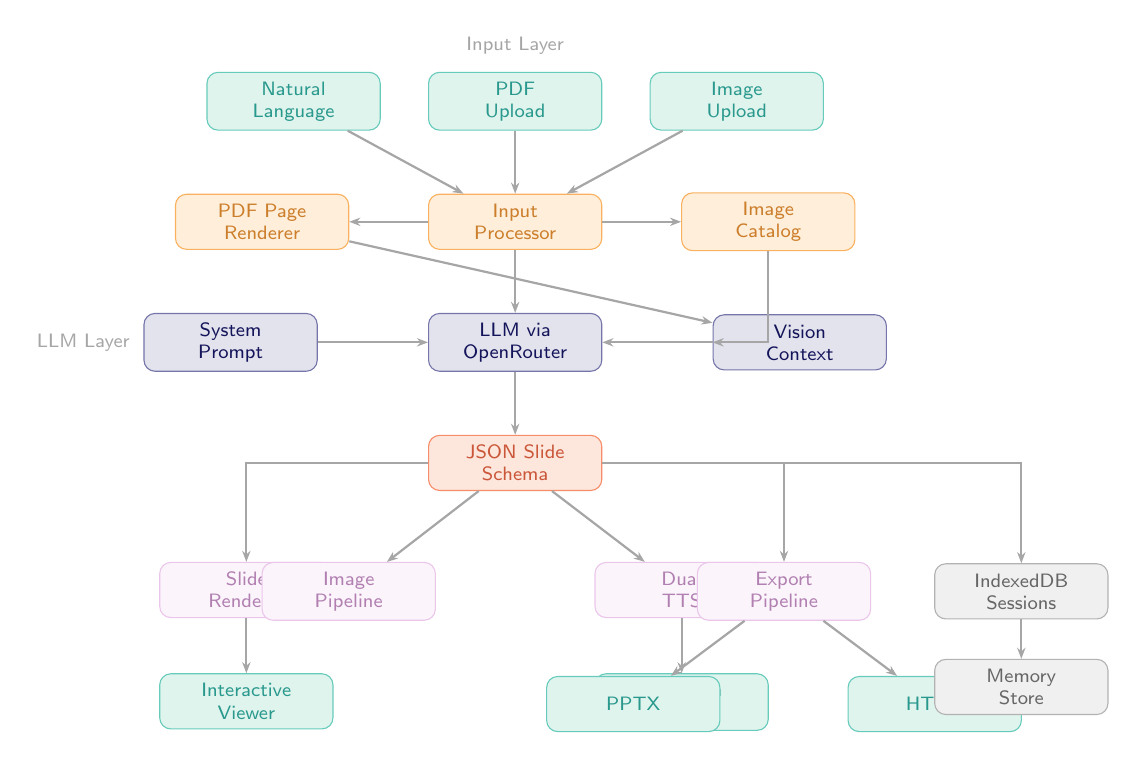
\begin{tikzpicture}[
    node distance=0.6cm and 1.0cm,
    box/.style={draw, rounded corners=4pt, minimum width=2.2cm, minimum height=0.7cm, align=center, font=\scriptsize\sffamily, fill=#1!12, draw=#1!60, text=#1!80!black},
    box/.default=MidnightBlue,
    arrow/.style={-{Stealth[length=4pt]}, thick, color=gray!70},
    label/.style={font=\scriptsize\sffamily, color=gray!70},
]

% ── Input Layer ──
\node[box=Emerald] (nl) {Natural\\Language};
\node[box=Emerald, right=0.6cm of nl] (pdf) {PDF\\Upload};
\node[box=Emerald, right=0.6cm of pdf] (img) {Image\\Upload};

% ── Processing ──
\node[box=BurntOrange, below=0.8cm of pdf] (proc) {Input\\Processor};
\node[box=BurntOrange, left=1.0cm of proc] (thumb) {PDF Page\\Renderer};
\node[box=BurntOrange, right=1.0cm of proc] (catalog) {Image\\Catalog};

% ── LLM ──
\node[box=MidnightBlue, below=0.8cm of proc] (llm) {LLM via\\OpenRouter};
\node[box=MidnightBlue, left=1.4cm of llm] (sys) {System\\Prompt};
\node[box=MidnightBlue, right=1.4cm of llm] (vision) {Vision\\Context};

% ── JSON ──
\node[box=RedOrange, below=0.8cm of llm] (json) {JSON Slide\\Schema};

% ── Render + Image + TTS + Export ──
\node[box=Plum, below left=0.9cm and 1.2cm of json] (render) {Slide\\Renderer};
\node[box=Plum, below left=0.9cm and -0.1cm of json] (imgpipe) {Image\\Pipeline};
\node[box=Plum, below right=0.9cm and -0.1cm of json] (tts) {Dual\\TTS};
\node[box=Plum, below right=0.9cm and 1.2cm of json] (export) {Export\\Pipeline};

% ── Outputs ──
\node[box=Emerald, below=0.7cm of render] (ui) {Interactive\\Viewer};
\node[box=Emerald, below=0.7cm of tts] (audio) {Narration\\+ Q\&A};
\node[box=Emerald, below left=0.7cm and -0.3cm of export] (pptx) {PPTX};
\node[box=Emerald, below right=0.7cm and -0.3cm of export] (html) {HTML};

% ── Storage ──
\node[box=Gray, right=0.8cm of export] (idb) {IndexedDB\\Sessions};
\node[box=Gray, below=0.5cm of idb] (mem) {Memory\\Store};

% ── Arrows ──
\draw[arrow] (nl) -- (proc);
\draw[arrow] (pdf) -- (proc);
\draw[arrow] (img) -- (proc);
\draw[arrow] (proc) -- (thumb);
\draw[arrow] (proc) -- (catalog);
\draw[arrow] (proc) -- (llm);
\draw[arrow] (thumb) -- (vision);
\draw[arrow] (catalog) |- (vision);
\draw[arrow] (sys) -- (llm);
\draw[arrow] (vision) -- (llm);
\draw[arrow] (llm) -- (json);
\draw[arrow] (json) -| (render);
\draw[arrow] (json) -- (imgpipe);
\draw[arrow] (json) -- (tts);
\draw[arrow] (json) -| (export);
\draw[arrow] (render) -- (ui);
\draw[arrow] (tts) -- (audio);
\draw[arrow] (export) -- (pptx);
\draw[arrow] (export) -- (html);
\draw[arrow] (json) -| (idb);
\draw[arrow] (idb) -- (mem);

% ── Layer labels ──
\node[label, above=0.1cm of pdf] {Input Layer};
\node[label, left=0.05cm of sys] {LLM Layer};

\end{tikzpicture}
\caption{High-level architecture of \system. User inputs (natural language, PDFs, images) are processed into a multimodal context for the LLM, which produces a structured JSON slide schema consumed by the renderer, image pipeline, TTS narration system, and export pipeline.}
\label{fig:architecture}
\end{figure}

\subsection{Stage 1: Research and Comprehension}

\system supports two co-equal input modes.
In \emph{document mode}, it renders each PDF page as a high-resolution image and includes it directly in the LLM's vision context, bypassing heuristic parsing entirely---the model sees the document as a human would, interpreting text, figures, tables, equations, and layout simultaneously.
In \emph{topic mode}, users describe a subject in natural language (e.g., ``Create a presentation on CRISPR gene editing''), and \sage curates content through web search, grounding the presentation in live, citable sources rather than relying solely on the model's training data.
The two modes can be combined: a user may upload a paper and enable web search to supplement it with recent developments.

An optional \emph{deep thinking mode} allocates an extended reasoning budget, allowing the model to spend more compute on content planning, source evaluation, and structural decisions before generating the slide JSON.
This is particularly valuable for complex or interdisciplinary topics where superficial treatment would miss important nuances.

\subsection{Stage 2: Structured Presentation Synthesis}

The LLM generates a structured JSON representation of the presentation, with each slide specifying a title, bullet-point content, a figure (SVG diagram, PDF crop, or image reference), layout directives, and speaker notes.
The separation of content from rendering is key: the LLM focuses on intellectual content while a deterministic renderer handles visual consistency.

Two aspects of this stage represent novel contributions:

\paragraph{SVG diagram synthesis.}
Rather than relying on stock images or templates, \system instructs the LLM to generate original inline SVG diagrams tailored to each slide's content.
A taxonomy of ten diagram types---flowcharts, comparison tables, timelines, layered architectures, Venn diagrams, network graphs, bar charts, annotated schematics, matrices, and cycle diagrams---with strict theme constraints (color palette, minimum font sizes, information density requirements) guides the generation.
This produces information-dense, content-specific visualizations rather than decorative graphics.

\paragraph{Vision-guided PDF figure extraction.}
When generating from an uploaded paper, the LLM can reference specific figures from the source document.
It predicts normalized bounding-box coordinates $[l, t, r, b] \in [0,1]^4$ for the target figure on a given page.
The system renders the page at high resolution, crops the specified region, and applies an automatic whitespace trimming algorithm that scans pixel values to produce tightly cropped results.
This eliminates the need for external figure detection models or heuristic PDF structure parsing.

\subsection{Stage 3: Streaming Slide Generation}

Unlike batch-mode systems that wait for the complete LLM response before displaying anything, \system renders slides incrementally as the model produces them.
An incremental JSON parser detects complete slide objects in the growing token stream and yields them to the renderer immediately.
The first slide typically appears within seconds, even for presentations that take 30--60 seconds to generate fully.
This reduces perceived latency, enables early user feedback, and allows interruption of unsatisfactory generations.

\subsection{Stage 4: Narrated Delivery}

\system transforms static slides into a narrated lecture experience through a dual text-to-speech pipeline.
Every slide includes LLM-generated speaker notes that reference the visible figure and guide the audience's attention.
A browser-native TTS engine (Web Speech API) provides zero-cost narration, while an optional neural TTS integration (Google Gemini) offers higher-quality voices, particularly for non-English content.
A prefetch buffering strategy fetches audio for the next slide while the current one is narrating, eliminating inter-slide gaps during auto-advance playback.

\subsection{Stage 5: Interactive Assessment}

After generation, users transition to a Q\&A mode where \sage answers questions about the presented content, grounded in the full slide context.
Users can ask comprehension questions (``explain the diagram on slide 3''), request elaboration on specific topics, or probe beyond what was presented.
This closes the loop from content delivery to knowledge verification, transforming \system from a one-shot generator into an interactive learning tool.

% ══════════════════════════════════════════════════════════
\section{Discussion and Future Work}
\label{sec:future}
% ══════════════════════════════════════════════════════════

\system demonstrates that modern LLMs are capable of generating complete, visually rich presentations from multimodal inputs with minimal human intervention.
The structured JSON approach provides a clean separation between creative content generation and deterministic rendering, and the SVG synthesis capability eliminates the need for a separate graphics pipeline.
The conversational paradigm---where users iteratively refine presentations through dialogue rather than one-shot generation---represents a meaningful departure from existing tools.

\paragraph{Content faithfulness and hallucination prevention.}
A fundamental concern for any system that generates educational content is \emph{faithfulness}: ensuring that presented information accurately reflects its sources rather than introducing fabricated claims.
\system addresses this through complementary mechanisms across both input modes.
In topic mode, web search grounds presentations in live, citable sources with inline references, reducing reliance on potentially stale training data.
In document mode, the vision-based pipeline provides the LLM with the full rendered document as context, reducing the risk of hallucination from incomplete input; PDF figure extraction further acts as evidence anchoring---rather than generating diagrams that \emph{describe} results, the system can embed the actual figures from the source paper.
Deep thinking mode contributes indirectly by allocating more reasoning to source evaluation and content planning, reducing rushed or superficial claims.
Nevertheless, LLM-generated content remains susceptible to subtle distortions, and we regard hallucination mitigation as a critical ongoing challenge.
Planned mitigations include integration of automated fact-checking through external verification APIs and a dedicated content-grounding mode that constrains the LLM to only make claims directly supported by its sources.

\paragraph{Socratic assessment and educational tools.}
A natural extension of the Q\&A feature is an \emph{assessment mode} in which \sage generates comprehension questions based on the presentation content and evaluates user responses.
We are actively exploring the integration of Socratic evaluation tools to strengthen \system's connection to the educational technology community.
This includes multiple-choice quiz generation derived from slide content, open-ended questions with LLM-graded rubrics calibrated against learning objectives, and Socratic dialogue that probes understanding through adaptive follow-up questions.
We envision this as particularly valuable in educational settings where students review AI-generated lecture presentations.
Recent work such as SlideBot~\citep{xie2026slidebot} demonstrates growing interest in grounding presentation generation in pedagogical theory; Socratic assessment would extend this direction by closing the loop from content delivery to comprehension verification.
We intend to implement and evaluate these capabilities prior to publication.

\paragraph{From comprehension to collaborative discovery.}
\system's current instantiation focuses on one end of the symbiotic loop's potential: helping humans comprehend existing knowledge more effectively.
But the iterative, bidirectional nature of the loop suggests a more ambitious trajectory.
When human and AI engage in sustained exchange---each questioning the other, each contributing complementary capabilities---the collaboration can generate novel ideas and connections that neither party would have reached alone.
We observe this phenomenon in our own development process: the conceptual framework presented in this paper, including the symbiotic loop itself, emerged through iterative human--AI dialogue rather than being designed \emph{a priori}.
Future work will explore whether \system can be extended beyond comprehension toward \emph{collaborative discovery}---supporting not just ``what does this paper say?'' but ``what does this paper \emph{not} say, and what should be investigated next?''
This direction connects to broader questions about whether human--AI symbiosis can fulfill Licklider's vision of partnerships that ``perform intellectual operations much more effectively than man alone can perform them''~\citep{licklider1960symbiosis}.

\paragraph{Democratizing tool creation through agentic coding.}
The development of \system itself illustrates a broader trend: the rise of agentic coding tools---AI assistants that can write, debug, and deploy software through conversational interaction---is lowering the barrier to creating personalized learning tools.
\system was built through such a process, with the symbiotic loop operating not only within the application but in the act of building it.
This suggests that the most profound impact of human--AI symbiosis for education may not be any single tool, but rather the democratization of tool creation: researchers, educators, and learners can increasingly build learning environments tailored to their own domains, pedagogical preferences, and workflows, without requiring traditional software engineering expertise.
We hope the community expands on this idea, using \system as a starting point or building entirely new tools---the open-source MIT license is chosen specifically to enable this.

Additional directions for future work include:

\paragraph{Collaborative editing.}
Users currently refine presentations through conversation (e.g., ``add a slide about X'' or ``change the diagram on slide 3'').
A direct-manipulation editing interface that allows users to modify slide content, rearrange slides, and adjust figures without returning to the chat would improve the iterative workflow.

\paragraph{Custom templates and branding.}
The current dark theme is fixed.
Supporting user-defined color palettes, font selections, and logo placement would enable institutional branding.

\paragraph{Accessibility.}
Adding ARIA attributes to the slide viewer, providing alt text for SVG diagrams (derived from figure labels and descriptions), and supporting screen reader navigation would improve accessibility.

\paragraph{Structured output with constrained decoding.}
Rather than relying entirely on prompt engineering for JSON conformance, integrating structured output modes~\citep{willard2023guided} available in newer model APIs could improve reliability and reduce the need for post-hoc JSON repair.

\paragraph{Migration to external TTS providers.}
While the dual Browser/Gemini TTS system substantially improves narration quality, dedicated speech synthesis services (e.g., NVIDIA Riva, OpenAI TTS, ElevenLabs) offer even higher quality voices with more natural prosody. Integration is planned once deployment and API key management constraints are resolved.


% ══════════════════════════════════════════════════════════
\section{Conclusion}
\label{sec:conclusion}
% ══════════════════════════════════════════════════════════

We have presented \system, an open-source platform that instantiates a \emph{symbiotic loop} between research curation, document understanding, and interactive learning.
Drawing on Licklider's vision of human--computer symbiosis~\citep{licklider1960symbiosis}, we have argued that framing the relationship between learner and AI as an iterative, bidirectional cycle---rather than a one-shot generation process---creates a more effective pathway from research to understanding.
By connecting web-grounded research curation with deep reasoning, vision-based document comprehension, structured presentation synthesis with custom SVG diagrams and extracted figures, streaming slide generation, dual-engine narrated delivery, and post-presentation Q\&A under a single conversational interface, \system unifies capabilities that have previously been studied in isolation.

The symbiotic loop is embodied in the \sage persona, which guides users from curiosity through comprehension assessment, with each iteration of the cycle deepening understanding.
The system's browser-based, bring-your-own-key architecture ensures accessibility, while its open-source MIT license invites community extension.

We have presented a detailed evaluation plan (Appendix~\ref{app:evaluation}) specifying five experiments that will provide quantitative evidence of the system's effectiveness across content quality, visual quality, figure extraction accuracy, workflow efficiency, and comparative performance.
These experiments, along with the integration of Socratic assessment tools and content faithfulness safeguards, will be completed prior to publication.

\system is available at \url{https://github.com/symbiont-ai/docent}, and we invite the community to build upon this work---particularly toward tighter integration with pedagogical frameworks, adaptive assessment, and hallucination-resistant educational content generation.
As agentic coding tools continue to mature, we envision a future in which researchers and educators routinely create their own AI-powered learning environments, tailored to their domains and pedagogical needs; \system and its open-source MIT license are offered as both a functional tool and a foundation for that vision.
While the current system targets comprehension of existing knowledge, the symbiotic loop framework points toward a more ambitious horizon: human--AI collaborative discovery, in which iterative bidirectional exchange produces not just understanding of what is known, but insight into what is not yet known.


% ══════════════════════════════════════════════════════════
% REFERENCES
% ══════════════════════════════════════════════════════════
\clearpage
\bibliography{references}


% ══════════════════════════════════════════════════════════
% APPENDICES
% ══════════════════════════════════════════════════════════
\appendix

\section{System Architecture}
\label{app:architecture}

\system is architected as a client-heavy web application with a thin server-side proxy, comprising six major subsystems: the input pipeline, the LLM integration layer, the rendering engine, the image enrichment pipeline, the narration system, and the export pipeline (see Figure~\ref{fig:architecture} in the main text).

\subsection{Input Processing Pipeline}

The input pipeline accepts three modalities:

\paragraph{Natural language.}
Users describe a topic in free text (e.g., ``Create a 10-slide presentation on CRISPR gene editing'').
The system applies intent detection heuristics---keyword matching and regex patterns over the user's message and recent conversation history---to determine whether a presentation generation request is being made.
Crucially, \system generates presentations in the user's language: prompts in Turkish, German, French, or any other language yield slides with content in that language, while internal AI instructions remain in English to ensure generation quality.

\paragraph{PDF documents.}
When a user uploads a PDF, the system dynamically loads \texttt{pdfjs-dist}~\citep{pdfjs2024} to parse the document.
Each page is rendered to an offscreen \texttt{<canvas>} element at high resolution (computed as a $16.67\times$ scale factor over the default 72 DPI).
The rendered pages are encoded as JPEG data URLs and transmitted to the LLM as image content blocks, enabling the model to visually comprehend text, figures, tables, equations, and layout.
Up to 30 pages are processed, providing comprehensive document coverage.
The system automatically routes between \emph{visual mode} (sending page images for figure-heavy content) and \emph{text mode} (extracting text for summarization tasks), optimizing cost and context usage.

\paragraph{Images.}
Uploaded images (PNG, JPEG, etc.) are registered in an image catalog with unique identifiers (e.g., \texttt{img\_upload\_0}).
The catalog is appended to the system prompt, enabling the LLM to reference uploaded images by ID and place them on semantically appropriate slides.

\subsection{LLM Integration}

\system communicates with LLMs through OpenRouter~\citep{openrouter2024}, a unified API gateway that provides access to models from multiple providers including Anthropic (Claude Sonnet~4, Claude Haiku~4), OpenAI (GPT-4o), Google (Gemini 2.5 Flash), Meta (Llama 3.3 70B), DeepSeek (DeepSeek V3), and Qwen (Qwen 2.5 Coder 32B).
The model picker allows users to browse all available OpenRouter models with capability tags, with configurable maximum output tokens that adapt to the selected model's limits.

The server-side component is a thin Next.js API route that translates client requests into the OpenRouter-compatible format, handling content block translation between Anthropic-style and OpenAI-style image formats, injecting provider preferences, and forwarding API keys.

Two optional modes enhance generation quality and are central to \system's role as a research curation tool:

\paragraph{Deep thinking mode.}
For complex or interdisciplinary presentations, the system enables extended reasoning with a configurable token budget (up to 40{,}000 reasoning tokens).
This allows the model to invest more compute in content planning---evaluating source quality, identifying the most pedagogically effective structure, resolving conceptual tensions across sources, and selecting appropriate diagram types---before committing to the JSON output.
Deep thinking is particularly valuable for topic-based generation, where the model must synthesize information from its training knowledge or retrieved web sources rather than following the structure of a single document.

\paragraph{Web search mode.}
The system integrates web search via OpenRouter's provider plugin mechanism, enabling \sage to ground presentations in live, citable sources.
In topic mode, web search is enabled by default, ensuring generated content reflects current information rather than relying solely on the model's training data.
In document mode, web search can be enabled alongside an uploaded PDF to supplement the paper with recent developments, related work, or broader context.
For chat-mode interactions, web search is available as a manual toggle, allowing users to ask \sage to look up specific claims or find additional references during the Q\&A stage.
Retrieved sources are included as inline references in speaker notes, providing traceability for every web-grounded claim.

\subsection{Rendering Engine}

The rendering engine consumes the structured JSON output and produces an interactive slide viewer implemented as a React component.
The renderer supports four layout modes:

\begin{itemize}[leftmargin=*,nosep]
    \item \textbf{Figure only}: The figure fills the entire slide body; no bullet points are shown.
    \item \textbf{Figure focus}: Bullet points occupy approximately 35\% of the width; the figure occupies 65\%.
    \item \textbf{Balanced}: An even 50/50 split between text and figure.
    \item \textbf{Text only}: No figure; full-width bullet points for introductory or concluding slides.
\end{itemize}

The layout is either explicitly specified in the JSON schema or automatically inferred: slides with no content default to \emph{figure only}, slides with three or fewer bullets default to \emph{figure focus}, and slides with more bullets default to \emph{balanced}.
A safety override ensures that \texttt{figure\_only} is promoted to \texttt{figure\_focus} whenever a slide contains content bullets, preventing text from being hidden.

SVG figures are rendered inline using \texttt{dangerouslySetInnerHTML} with automatic viewport normalization.
A ref callback inspects each SVG element, ensures \texttt{width}/\texttt{height} and \texttt{viewBox} attributes are present, and sets \texttt{preserveAspectRatio} to \texttt{xMidYMid meet} for proper scaling.

\subsection{Image Enrichment Pipeline}
\label{sec:images}

Beyond LLM-generated SVG diagrams and PDF figure crops, \system supports two additional modes of visual content:

\paragraph{AI image generation.}
Users can request AI-generated images for any slide via Gemini or Nano Banana models accessed through OpenRouter.
A prompt editor allows users to review and modify the generation prompt before sending.
Generated images replace the slide's SVG diagram, with the original SVG and speaker notes preserved for one-click revert.

\paragraph{Real photo search.}
A ``Find Photo'' feature searches the web for real photographs matching a query, proxies the results to avoid CORS restrictions, and embeds them directly into slides.
This is particularly useful for presentations requiring photographic content (e.g., travel, biology, architecture).

Both modes support a \textbf{revert-to-original} operation that restores the LLM-generated SVG, speaker notes, and references, enabling non-destructive experimentation with visual alternatives.

\subsection{PDF Figure Extraction Pipeline}
\label{sec:pdfcrop}

When a presentation is generated from an uploaded PDF, the LLM may reference specific figures, tables, or diagrams from the source document.
\system supports this through a \texttt{pdf\_crop} figure type, where the LLM specifies a page number and a normalized bounding box $[l, t, r, b]$ with each coordinate in $[0, 1]$.

The extraction pipeline operates as follows:

\begin{enumerate}[leftmargin=*,nosep]
    \item The target page is rendered at $3\times$ scale to an offscreen canvas using \texttt{pdfjs-dist}.
    \item The normalized coordinates are mapped to pixel coordinates: $x = l \cdot W$, $y = t \cdot H$, etc.
    \item The specified region is copied to a new canvas.
    \item An automatic whitespace trimming algorithm scans pixels (every 4th pixel for efficiency) with a white threshold of 245, identifies the bounding box of non-white content, adds a 2\% margin, and produces a tightly cropped result.
    \item The cropped image is encoded as a PNG data URL and cached by page-region key to avoid redundant rendering.
\end{enumerate}

Named region presets (e.g., \texttt{top\_half}, \texttt{left\_column}, \texttt{bottom\_third}) are also available for coarse-grained selections.


% ══════════════════════════════════════════════════════════

\section{Methodology}
\label{app:methodology}


\subsection{Presentation Generation via Prompt Engineering}

The core of \system's generation capability lies in a carefully designed system prompt that defines the presentation schema, figure types, diagram taxonomy, layout heuristics, and quality constraints.
This prompt is appended to the LLM's system message for every conversation in which presentation generation may occur.

The prompt specifies a JSON schema with the following structure per slide:

\begin{lstlisting}[language=json,caption={Slide JSON schema (simplified).},label={lst:schema}]
{
  "title": "Presentation Title",
  "slides": [
    {
      "title": "Slide Title",
      "content": ["Bullet point 1", "Bullet point 2"],
      "figure": {
        "type": "svg",
        "content": "<svg ...>...</svg>",
        "label": "Figure description"
      },
      "layout": "figure_focus",
      "speakerNotes": "Narration text for this slide."
    }
  ]
}
\end{lstlisting}

This schema separates content from presentation, enabling the rendering engine to apply consistent visual styling while the LLM focuses on content quality and figure selection.
The figure type field supports four values: \texttt{svg} for LLM-generated diagrams, \texttt{pdf\_crop} for figures extracted from uploaded PDFs, \texttt{image\_ref} for images from the uploaded image catalog, and \texttt{card} for styled text cards when a diagram is not appropriate.

\subsubsection{Slide Count Enforcement}

A persistent challenge with LLM-generated presentations is delivering the exact number of slides requested by the user.
\system addresses this through a multi-pronged approach:

\begin{enumerate}[leftmargin=*,nosep]
    \item The system prompt specifies an explicit formula: for $N$ requested content slides, the JSON must contain exactly $N+3$ slides (1~title + $N$~content + 1~references + 1~closing).
    \item Concrete worked examples (e.g., ``5 slides $\rightarrow$ 8 total'') are provided in the prompt.
    \item A regex-based count reminder is injected as an additional user message when a specific slide count is detected in the user's request.
\end{enumerate}

\subsection{SVG Diagram Synthesis}
\label{sec:svg}

A distinguishing feature of \system is its use of LLM-generated inline SVG diagrams as the primary visual content for slides.
Rather than relying on stock images or template-based graphics, the system instructs the LLM to generate SVG markup tailored to each slide's specific content.

The system prompt defines ten diagram types, each with usage guidance:

\begin{enumerate}[leftmargin=*,nosep]
    \item \textbf{Flowchart / Pipeline}: Rectangular nodes connected by arrows for methods, protocols, and workflows.
    \item \textbf{Comparison Table}: Grid layouts with colored headers for feature matrices and method comparisons.
    \item \textbf{Timeline}: Horizontal or vertical lines with milestone markers for chronological information.
    \item \textbf{Layered Architecture}: Stacked horizontal rectangles for software stacks and hierarchical structures.
    \item \textbf{Venn / Overlap}: Semi-transparent overlapping circles for relationships and intersections.
    \item \textbf{Network / Hub-Spoke}: Central nodes with radiating connections for interactions and communication.
    \item \textbf{Bar Chart / Metrics}: Proportional rectangles with value labels for quantitative comparisons.
    \item \textbf{Annotated Schematic}: Simplified illustrations with labeled callout lines for structural components.
    \item \textbf{Matrix / Heatmap}: Color-intensity grids for correlation data and scoring.
    \item \textbf{Cycle / Circular}: Nodes in circular arrangement with curved arrows for iterative processes and feedback loops.
\end{enumerate}

The prompt further imposes quality constraints:

\begin{itemize}[leftmargin=*,nosep]
    \item \textbf{Theme consistency}: All SVGs must use a dark theme palette---background \texttt{\#1A2332}, text \texttt{\#E8EAED}, accents \texttt{\#D4A853}, \texttt{\#5BB8D4}, \texttt{\#6BC485}, \texttt{\#D46B6B}, \texttt{\#A78BFA}---ensuring visual coherence with the slide template.
    \item \textbf{Information density}: Diagrams must include specific numbers, names, and details, not generic placeholder boxes.
    \item \textbf{Readability}: Minimum font size of 13px, bold headings within SVG, and 40px padding from edges.
    \item \textbf{Technical correctness}: Single quotes for all SVG attributes (to avoid breaking JSON parsing), proper XML entity encoding (\texttt{\&amp;} instead of bare \texttt{\&}), and minimum viewBox dimensions of $800 \times 500$.
    \item \textbf{Visual polish}: Rounded corners (\texttt{rx='8'}), 3--5 accent colors per diagram, and reusable arrow markers via \texttt{<defs>}.
    \item \textbf{Diversity}: The prompt explicitly instructs the LLM to vary diagram types across slides, avoiding repetitive use of a single style.
\end{itemize}

\subsection{Speaker Notes and Narration}
\label{sec:narration}

Every content slide includes a \texttt{speakerNotes} field containing narration text.
The system prompt instructs the LLM to write notes that reference the visible figure, point out specific details, and guide the audience's attention.
Speaker notes are \textbf{editable inline} in the slide viewer, with debounced auto-save to IndexedDB (500ms delay) and a revert option to restore AI-generated originals.

\system implements a \textbf{dual TTS pipeline}:

\paragraph{Browser TTS (free).}
The Web Speech API's \texttt{SpeechSynthesisUtterance} is used with language-aware voice selection.
Markdown formatting is stripped from text, which is then split into chunks of approximately 180 characters at sentence boundaries.
Each chunk is spoken sequentially with an 80ms gap.
Voice selection is configurable (female, male, neutral) with preferred voice lists and English-language fallbacks.
A generation counter prevents stale utterances from playing after navigation or cancellation.

\paragraph{Gemini AI TTS (optional).}
For higher-quality narration---particularly for non-English languages where browser voices are often poor---an optional Google Gemini TTS integration provides neural voices.
The system implements \textbf{prefetch buffering}: while the current slide is narrating, audio for the next slide is fetched in advance.
This look-ahead strategy eliminates perceptible gaps between slides during auto-advance narration.

An \textbf{auto-advance} mode plays through all slides automatically, transitioning to the next slide when the current slide's narration completes.
An \textbf{auto-voice} mode can optionally narrate every chat response, not just slide content.

\subsection{Presentation Q\&A}
\label{sec:qa}

After generating a presentation, users can enter a Q\&A mode where \sage answers questions about the slide content.
The system maintains full context of all slides and tracks which slide the user is currently viewing.
Queries like ``What's on slide 3?'' or ``Explain the diagram on this slide'' are resolved using slide-index detection in the user's message.
This transforms \system from a one-shot generator into an interactive learning tool.


% ══════════════════════════════════════════════════════════

\section{Implementation}
\label{app:implementation}


\subsection{Technology Stack}

\system is implemented as a Next.js application (version~16) using React~19 and TypeScript.
Table~\ref{tab:stack} summarizes the key dependencies.

\begin{table}[t]
\centering
\caption{Technology stack and key dependencies.}
\label{tab:stack}
\begin{tabular}{@{}lll@{}}
\toprule
\textbf{Component} & \textbf{Technology} & \textbf{Purpose} \\
\midrule
Framework & Next.js 16 / React 19 & Application shell, routing, API routes \\
Language & TypeScript 5.9 & Type-safe development \\
PDF Processing & pdfjs-dist 5.4 & PDF parsing, rendering, figure cropping \\
PPTX Export & PptxGenJS 4.0 & PowerPoint file generation \\
Storage & idb-keyval / IndexedDB & Browser-local session persistence \\
Charts & Recharts 3.7 & Optional data visualization \\
Speech (free) & Web Speech API & Browser-native TTS narration \\
Speech (neural) & Google Gemini API & High-quality neural TTS \\
LLM Gateway & OpenRouter API & Multi-model LLM access \\
\bottomrule
\end{tabular}
\end{table}

\subsection{Multi-Model Support}

Via OpenRouter~\citep{openrouter2024}, \system provides access to all available models, with a curated default set spanning six providers:

\begin{itemize}[leftmargin=*,nosep]
    \item \textbf{Anthropic}: Claude Sonnet~4 (default), Claude Haiku~4
    \item \textbf{OpenAI}: GPT-4o, GPT-4o Mini
    \item \textbf{Google}: Gemini 2.5 Flash
    \item \textbf{Meta}: Llama 3.3 70B
    \item \textbf{DeepSeek}: DeepSeek V3
    \item \textbf{Qwen}: Qwen 2.5 Coder 32B
\end{itemize}

A model picker allows users to browse all available models with capability tags.
The maximum output tokens slider adapts to the selected model's limits, ensuring users do not exceed context constraints.

\subsection{Session, State, and Memory Management}

\system maintains rich client-side state through a composition of React hooks:

\begin{itemize}[leftmargin=*,nosep]
    \item \texttt{useChat}: Orchestrates message flow, file uploads, API calls, and coordinates all sub-hooks.
    \item \texttt{usePresentation}: Manages slide state, navigation, and figure resolution (including image catalog lookups).
    \item \texttt{usePDF}: Handles PDF loading, page rendering, thumbnail generation, and figure cropping.
    \item \texttt{useTTS}: Manages dual speech synthesis with voice selection, chunked playback, and prefetch buffering.
    \item \texttt{useMemory}: Extracts and persists user-specific notes for cross-session context via \texttt{[NOTE:]} tags in LLM responses.
    \item \texttt{useSessions}: Serializes and restores complete session state to/from IndexedDB, with auto-save after every interaction.
\end{itemize}

Sessions capture conversation history, uploaded file metadata, presentation state (slides, current position), and PDF viewer state (page, zoom level), enabling users to resume work across browser sessions.
The memory system allows \sage to accumulate knowledge about user preferences across sessions---for instance, preferred diagram styles, domain-specific terminology, or presentation conventions---without requiring server-side user accounts.

\subsection{Robust JSON Parsing}

A practical challenge in LLM-based structured generation is handling malformed or truncated JSON output.
\system implements a multi-stage repair pipeline:

\begin{enumerate}[leftmargin=*,nosep]
    \item Standard JSON parsing of code-fenced blocks.
    \item SVG-aware repair: SVG elements within JSON often contain double quotes that break parsing; the system identifies SVG ranges and replaces internal double quotes with single quotes before re-parsing.
    \item Truncation repair: For responses cut off mid-generation, the system locates the last complete slide object and attempts to close the JSON structure with progressively aggressive bracket sequences.
\end{enumerate}

This pipeline ensures that even partially generated presentations---common when model output limits are reached---can be displayed to the user.

\subsection{Streaming Slide Generation}
\label{sec:streaming}

Rather than waiting for the LLM to generate the complete JSON response before displaying any content, \system implements streaming slide generation that renders slides incrementally as they are produced.
The system reads the LLM's response token by token and applies an incremental JSON parser that detects when a complete slide object has been emitted.
Each time a new slide boundary is identified, the slide is immediately parsed, rendered, and appended to the presentation viewer, allowing the user to begin reviewing early slides while later slides are still being generated.

This approach provides several benefits.
First, perceived latency is dramatically reduced: the first slide typically appears within seconds, even for long presentations that may take 30--60 seconds to generate fully.
Second, users can begin reading and evaluating content immediately, enabling early decisions about whether to interrupt generation (via a cancel button) and adjust the prompt.
Third, the streaming approach composes naturally with the truncation repair mechanism described above---if generation is interrupted or hits a token limit, all slides completed up to that point are already visible and usable.

The implementation extends the robust JSON parsing pipeline with a sliding-window approach: as tokens accumulate, the parser attempts to extract complete slide objects from the growing buffer, yielding them to the renderer as soon as they validate.

\subsection{Export Pipeline}

\system supports two export formats:

\paragraph{PowerPoint (PPTX).}
The system uses PptxGenJS~\citep{pptxgenjs2024} to construct PowerPoint files programmatically.
SVG figures are first rasterized to PNG via an offscreen canvas pipeline: the SVG is base64-encoded, loaded into an \texttt{Image} element, drawn onto a $960 \times 540$ canvas, and exported as a PNG data URL.
PDF crops are embedded directly as PNG images.
Speaker notes are attached to slides when enabled.
AI-generated background images are included on title slides.

\paragraph{Self-contained HTML.}
An alternative export generates a single HTML file with inline CSS, embedded navigation, and branding that can be opened in any browser and printed to PDF.
All SVG figures are embedded inline, and all raster images are included as base64 data URLs, producing a fully self-contained document with no external dependencies.




% ══════════════════════════════════════════════════════════
\section{Evaluation Plan}
\label{app:evaluation}
% ══════════════════════════════════════════════════════════


We report on qualitative observations from development testing and present a detailed plan for systematic evaluation experiments.
All planned experiments described below will be completed and their results reported prior to publication.
We deliberately refrain from reporting quantitative metrics that have not yet been measured, but commit to executing each experiment as specified.

\subsection{Qualitative Observations from Development Testing}

During iterative development, we have observed the following patterns across informal testing with diverse topics and PDF documents:

\begin{itemize}[leftmargin=*,nosep]
    \item \textbf{SVG rendering quality} varies substantially across models. Vision-capable models (Claude Sonnet~4, GPT-4o, Gemini) consistently produce well-formed SVG with correct attribute quoting, proper use of the color palette, and readable text labels. Smaller models (Llama 3.3 70B, Qwen 2.5 Coder 32B) occasionally produce SVGs with minor rendering artifacts such as overlapping text or missing arrow markers.
    \item \textbf{PDF figure extraction} generally succeeds for well-structured papers. The most common failure mode is over-extending the bottom crop coordinate to include caption text. The whitespace trimming algorithm mitigates this in many cases.
    \item \textbf{JSON reliability} varies by model. Larger models rarely produce unparseable output, while smaller models occasionally generate malformed JSON, which the multi-stage repair pipeline usually recovers.
    \item \textbf{Multilingual generation} works reliably for major languages (tested informally with Turkish, German, French, Spanish) with content quality comparable to English output for well-resourced languages (Figure~\ref{fig:multilingual-ui}). Browser TTS quality for non-English languages is poor; Gemini TTS substantially improves non-English narration quality.
    \item \textbf{Slide count adherence} has improved with the multi-pronged enforcement approach, but models occasionally generate one fewer or one more content slide than requested.
\end{itemize}

These observations, while informative, are anecdotal and lack the controlled methodology needed for rigorous claims.
The following subsections specify the experiments that will provide quantitative evidence.

\begin{figure*}[t]
\centering
\includegraphics[width=\textwidth]{docent_multilingual_ui.png}
\caption{\system interface showing a Quantum Computing presentation with custom SVG diagrams (superposition, entanglement, and exponential scaling visualizations), inline references, editable speaker notes, and narration/Q\&A controls. The session sidebar (left) demonstrates multilingual generation across five languages: English, Spanish, French, German, and Turkish.}
\label{fig:multilingual-ui}
\end{figure*}

\subsection{Planned Experiment 1: Content Quality and Factual Accuracy}
\label{sec:eval-content}

\paragraph{Objective.}
Assess the factual accuracy and content coverage of generated presentations across diverse domains and input modalities.

\paragraph{Test corpus.}
We will assemble a corpus of 20 evaluation inputs spanning two modalities:

\begin{itemize}[leftmargin=*,nosep]
    \item \textbf{Topic mode} (10 topics): Five well-established academic domains (molecular biology, computer science, economics, art history, climate science) $\times$ two specificity levels (broad: ``Introduction to machine learning''; narrow: ``Transformer attention mechanisms'').
    \item \textbf{PDF mode} (10 papers): Papers selected from diverse domains and venues, including both single-column and two-column layouts, and papers with varying figure density.
\end{itemize}

\paragraph{Metrics.}
For each generated presentation, human evaluators will rate on 1--5 Likert scales:

\begin{enumerate}[leftmargin=*,nosep]
    \item \textbf{Factual accuracy}: Are claims on slides correct and verifiable?
    \item \textbf{Coverage}: Does the presentation capture the key themes, methods, and conclusions of the source material?
    \item \textbf{Narrative coherence}: Do slides follow a logical progression?
    \item \textbf{Speaker notes quality}: Are narration scripts natural, informative, and aligned with visible slide content?
\end{enumerate}

Additionally, we will use LLM-as-a-judge~\citep{zheng2024judging} as a scalable complement to human evaluation, prompting a separate model to rate presentations on the same dimensions and measuring inter-rater agreement between human and automated judges.

\paragraph{Baselines.}
Each PDF-mode input will also be presented manually by a domain-knowledgeable human, providing a manual-creation baseline for comparison.

\subsection{Planned Experiment 2: Visual Quality and Diagram Diversity}
\label{sec:eval-visual}

\paragraph{Objective.}
Measure the quality, diversity, and rendering correctness of LLM-generated SVG diagrams.

\paragraph{Protocol.}
From the 20 test presentations (expected to yield approximately 150--200 content slides), we will analyze every generated SVG diagram for:

\begin{enumerate}[leftmargin=*,nosep]
    \item \textbf{Diagram type distribution}: Frequency of each of the ten diagram types across the corpus.
    \item \textbf{Rendering correctness}: Whether the SVG renders without artifacts (overlapping text, missing elements, broken arrows, viewport overflow). Binary pass/fail per diagram.
    \item \textbf{Information density}: Whether the diagram contains domain-specific data (numbers, names, labels) rather than generic placeholders. Binary pass/fail.
    \item \textbf{Theme compliance}: Whether colors, fonts, and spacing adhere to the specified dark-theme palette. Binary pass/fail.
\end{enumerate}

\paragraph{Model comparison.}
We will run the same 20 inputs through three models---Claude Sonnet~4, GPT-4o, and Gemini 2.5 Flash---and compare rendering correctness rates and diagram type distributions across models.

\subsection{Planned Experiment 3: PDF Figure Extraction Accuracy}
\label{sec:eval-pdfcrop}

\paragraph{Objective.}
Quantify the accuracy of the vision-guided PDF figure extraction pipeline.

\paragraph{Protocol.}
For each of the 10 PDF-mode test papers, we will:

\begin{enumerate}[leftmargin=*,nosep]
    \item Manually annotate all figures and tables with ground-truth bounding boxes.
    \item Generate a presentation and record the LLM-predicted crop coordinates for each referenced figure.
    \item Compute Intersection over Union (IoU) between predicted and ground-truth bounding boxes.
    \item Classify extraction outcomes: \emph{correct} (IoU $> 0.7$ and no extraneous content), \emph{acceptable} (IoU $> 0.5$, minor inclusion of captions or adjacent text), and \emph{failed} (IoU $< 0.5$ or wrong figure entirely).
\end{enumerate}

\paragraph{Analysis.}
We will report per-paper and aggregate accuracy, analyze failure modes (caption inclusion, wrong figure, coordinate miscalibration), and assess the effectiveness of the automatic whitespace trimming as a post-processing correction.

\subsection{Planned Experiment 4: Workflow Efficiency}
\label{sec:eval-time}

\paragraph{Objective.}
Measure end-to-end generation time and compare against manual creation.

\paragraph{Protocol.}
For a subset of 5 inputs, we will:

\begin{enumerate}[leftmargin=*,nosep]
    \item Time the end-to-end generation from user submission to fully rendered slides, broken down by phase: PDF rendering, LLM generation, JSON parsing, slide rendering.
    \item Ask 3 domain-knowledgeable volunteers to manually create equivalent presentations (same topic, comparable visual quality) and record their preparation time.
    \item Compute the time ratio between automated and manual creation.
\end{enumerate}

\subsection{Planned Experiment 5: Comparative System Evaluation}
\label{sec:eval-comparison}

\paragraph{Objective.}
Compare \system against the closest available systems on a standardized task.

\paragraph{Protocol.}
We will select 5 inputs (3 topic-mode, 2 PDF-mode) and generate presentations using \system, Gamma, and Canva (commercial tools).
For academic comparison, we will also evaluate against PPTAgent~\citep{zheng2025pptagent} and SlideTailor~\citep{zeng2026slidetailor} where feasible (both require reference presentations or example pairs as input, which differs from \system's from-scratch generation paradigm).
Human evaluators will rate all outputs on content quality, visual quality, and overall preference using a blind evaluation protocol (system identity hidden).

\paragraph{Adoption of PPTEval.}
Where applicable, we will report PPTEval~\citep{zheng2025pptagent} scores (Content, Design, Coherence) for comparability with prior work.

\begin{table}[H]
\centering
\scriptsize
\caption{Feature comparison of \system with AI presentation tools.
\checkmark\ = fully supported, $\sim$ = partial support, -- = not supported.
Systems are grouped into open-source/academic (left) and commercial (right).}
\label{tab:comparison}
\renewcommand{\arraystretch}{0.92}
\begin{tabularx}{\textwidth}{@{} >{\raggedright\arraybackslash}p{1.8cm} >{\raggedright\arraybackslash}X c c c c c c c c @{}}
\toprule
& & \multicolumn{4}{c}{\textbf{Open-Source / Academic}} & \multicolumn{4}{c}{\textbf{Commercial}} \\
\cmidrule(lr){3-6} \cmidrule(lr){7-10}
\textbf{Feature}
  & \textbf{Description}
  & \rotatebox{70}{\textbf{Docent}}
  & \rotatebox{70}{\textbf{PPTAgent}}
  & \rotatebox{70}{\textbf{SlideTailor}}
  & \rotatebox{70}{\textbf{Presenton}}
  & \rotatebox{70}{\textbf{Beautiful.ai}}
  & \rotatebox{70}{\textbf{Gamma}}
  & \rotatebox{70}{\textbf{Canva}}
  & \rotatebox{70}{\textbf{SlidesAI}} \\
\midrule
\multicolumn{10}{@{}l}{\textit{Interaction \& Research}} \\[1pt]
Conversational refinement
  & Modify presentations via dialogue or direct UI editing
  & \checkmark & -- & -- & -- & $\sim$ & $\sim$ & $\sim$ & -- \\
Web search
  & Retrieves live web sources to ground slide content in current information
  & \checkmark & -- & -- & -- & -- & -- & -- & -- \\
Deep thinking / research
  & Extended reasoning or multi-step agentic research before generation
  & \checkmark & -- & -- & -- & -- & -- & -- & -- \\
Post-generation Q\&A
  & Comprehension or follow-up questions after presentation, answered by LLM
  & \checkmark & -- & -- & -- & -- & -- & -- & -- \\
Personalized preferences
  & User-specific preferences for content, structure, or visual style
  & $\sim$ & -- & \checkmark & -- & -- & -- & -- & -- \\
\midrule
\multicolumn{10}{@{}l}{\textit{Content Generation}} \\[1pt]
Custom SVG diagrams
  & LLM generates original vector diagrams (flowcharts, timelines, etc.) per slide
  & \checkmark & -- & -- & -- & -- & -- & -- & -- \\
PDF figure extraction
  & Crops figures from uploaded PDFs via vision-based coordinate prediction
  & \checkmark & -- & -- & -- & -- & -- & -- & -- \\
Vision-based PDF reading
  & Renders PDF pages as images for multimodal LLM analysis without heuristic parsing
  & \checkmark & -- & -- & -- & -- & -- & -- & -- \\
AI image generation
  & Text-to-image models (DALL-E, Stable Diffusion) for custom slide imagery
  & \checkmark & -- & -- & \checkmark & -- & \checkmark & \checkmark & -- \\
Real photo search
  & Searches stock photo APIs (Pexels, Unsplash, Pixabay) for relevant imagery
  & \checkmark & -- & -- & \checkmark & -- & \checkmark & \checkmark & -- \\
\midrule
\multicolumn{10}{@{}l}{\textit{Architecture \& Flexibility}} \\[1pt]
Multi-model (BYOK)
  & Multiple LLM providers via user-supplied API keys; not locked to one vendor
  & \checkmark & $\sim$ & $\sim$ & \checkmark & -- & -- & -- & -- \\
Structured JSON schema
  & Defined schema for slides; deterministic rendering separate from generation
  & \checkmark & \checkmark & \checkmark & -- & $\sim$ & -- & -- & -- \\
Streaming generation
  & Slides render incrementally as the LLM produces them
  & \checkmark & -- & -- & -- & -- & -- & -- & -- \\
Browser-only (zero install)
  & Runs in the browser with no server or installation required
  & \checkmark & -- & -- & -- & \checkmark & \checkmark & \checkmark & $\sim$ \\
Open source
  & Full source code publicly available under an open-source license
  & \checkmark & \checkmark & \checkmark & \checkmark & -- & -- & -- & -- \\
Multi-language
  & Generates presentations and conducts dialogue in non-English languages
  & \checkmark & -- & $\sim$ & -- & -- & $\sim$ & $\sim$ & $\sim$ \\
\midrule
\multicolumn{10}{@{}l}{\textit{Presentation \& Delivery}} \\[1pt]
Speaker notes + TTS
  & Auto-generates speaker notes per slide with text-to-speech narration
  & \checkmark & -- & -- & -- & -- & -- & -- & -- \\
PPTX export
  & Exports to editable Microsoft PowerPoint format
  & \checkmark & \checkmark & \checkmark & \checkmark & \checkmark & \checkmark & \checkmark & \checkmark \\
PDF/HTML export
  & Exports to PDF or standalone HTML formats
  & \checkmark & -- & -- & \checkmark & \checkmark & \checkmark & \checkmark & -- \\
Evaluation framework
  & Systematic benchmark or metric suite for assessing presentation quality
  & -- & \checkmark & \checkmark & -- & -- & -- & -- & -- \\
\bottomrule
\end{tabularx}
\end{table}

\begin{table}[H]
\centering
\scriptsize
\caption{Comparison of academic presentation generation systems.
\emph{Input}: what the system requires beyond the target document.
\emph{Approach}: whether the system trains task-specific parameters (Trained) or orchestrates pre-trained LLMs via prompting (Prompting).
\emph{Interaction}: whether the user can refine outputs through dialogue (Conv.) or only receives a one-shot batch output.}
\label{tab:academic}
\renewcommand{\arraystretch}{1.15}
\setlength{\tabcolsep}{3pt}
\begin{tabularx}{\textwidth}{@{} >{\raggedright\arraybackslash}p{2.1cm} c >{\raggedright\arraybackslash}X c c c c @{}}
\toprule
\textbf{System}
  & \textbf{Venue}
  & \textbf{Primary Input}
  & \textbf{Approach}
  & \textbf{Interact.}
  & \textbf{Output}
  & \textbf{Eval.} \\
\midrule
Doc2PPT \newline{\scriptsize\citep{fu2022doc2ppt}}
  & AAAI '22
  & Doc
  & Trained
  & Batch
  & Slides
  & Custom \\
PPTAgent \newline{\scriptsize\citep{zheng2025pptagent}}
  & EMNLP '25
  & Doc + ref.\ slides
  & Prompting
  & Batch
  & PPTX
  & PPTEval \\
AutoPresent \newline{\scriptsize\citep{ge2025autopresent}}
  & CVPR '25
  & Instructions
  & Hybrid
  & Batch
  & PPTX
  & SlidesBench \\
PresentAgent \newline{\scriptsize\citep{wu2025presentagent}}
  & EMNLP '25
  & Doc
  & Prompting
  & Batch
  & Video
  & PresentEval \\
SlideBot \newline{\scriptsize\citep{xie2026slidebot}}
  & EAAI '26
  & Topic (retrieval)
  & Prompting
  & Batch
  & Beamer
  & User study \\
SlideTailor \newline{\scriptsize\citep{zeng2026slidetailor}}
  & AAAI '26
  & Doc + example + template
  & Prompting
  & Batch
  & PPTX
  & PSP \\
SlideGen \newline{\scriptsize\citep{liang2025slidegen}}
  & arXiv '25
  & Doc
  & Prompting
  & Batch
  & PPTX
  & GAD \\
\midrule
\textbf{Docent} (ours)
  & --
  & Topic \emph{or} doc
  & Prompting
  & Conv.+stream
  & Interactive + TTS
  & Planned \\
\bottomrule
\end{tabularx}
\setlength{\tabcolsep}{6pt}
\end{table}

\begin{table}[H]
\centering
\scriptsize
\caption{Feature comparison of \system with educational and research AI tools.
\checkmark\ = fully supported, $\sim$ = partial support, -- = not supported.
Rows are ordered to reflect the research-to-presentation workflow.}
\label{tab:comparison-edu}
\renewcommand{\arraystretch}{1.05}
\begin{tabularx}{\textwidth}{@{} >{\raggedright\arraybackslash}p{1.8cm} >{\raggedright\arraybackslash}X c c c c c @{}}
\toprule
& & \multicolumn{2}{c}{\textbf{Open-Source / Academic}} & \multicolumn{3}{c}{\textbf{Commercial}} \\
\cmidrule(lr){3-4} \cmidrule(lr){5-7}
\textbf{Feature}
  & \textbf{Description}
  & \rotatebox{70}{\textbf{Docent}}
  & \rotatebox{70}{\textbf{SlideBot}}
  & \rotatebox{70}{\textbf{NotebookLM}}
  & \rotatebox{70}{\textbf{Perplexity}}
  & \rotatebox{70}{\textbf{SciSpace}} \\
\midrule
\multicolumn{7}{@{}l}{\textit{Research \& Document Analysis}} \\[1pt]
Document / PDF Q\&A
  & Conversational question-answering over uploaded documents with source-grounded responses
  & \checkmark & -- & \checkmark & \checkmark & \checkmark \\
Web search
  & Retrieves live web sources to ground content in current information
  & \checkmark & $\sim$ & \checkmark & \checkmark & \checkmark \\
Deep thinking / research
  & Extended reasoning for content planning, or multi-step agentic research across sources
  & \checkmark & $\sim$ & \checkmark & \checkmark & -- \\
Source-grounded citations
  & Responses include inline citations linking to specific passages in source documents
  & $\sim$ & \checkmark & \checkmark & \checkmark & \checkmark \\
PDF figure extraction
  & Extracts, crops, or explains figures, tables, and equations from uploaded PDF documents
  & \checkmark & \checkmark & -- & -- & \checkmark \\
Academic corpus search
  & Searches large scholarly databases (e.g., Semantic Scholar, arXiv) for relevant literature
  & -- & \checkmark & -- & $\sim$ & \checkmark \\
\midrule
\multicolumn{7}{@{}l}{\textit{Presentation Generation}} \\[1pt]
Slide generation
  & Produces complete slide decks from documents, topics, or research results
  & \checkmark & \checkmark & \checkmark & \checkmark & -- \\
Custom SVG diagrams
  & LLM generates original vector diagrams (flowcharts, timelines, architectures) per slide
  & \checkmark & -- & -- & -- & -- \\
Conversational refinement
  & Modify presentations via dialogue or direct UI editing of slides, images, and speaker notes
  & \checkmark & $\sim$ & -- & $\sim$ & -- \\
PPTX export
  & Exports to editable Microsoft PowerPoint format
  & \checkmark & -- & -- & \checkmark & -- \\
\midrule
\multicolumn{7}{@{}l}{\textit{Educational \& Assessment}} \\[1pt]
Post-generation Q\&A
  & Users ask comprehension or follow-up questions about the presented content
  & \checkmark & -- & \checkmark & $\sim$ & $\sim$ \\
Quiz / flashcard generation
  & Automatically generates quizzes, flashcards, or study materials from source content
  & -- & -- & \checkmark & -- & -- \\
Audio overview / TTS
  & Generates audio summaries or narrated delivery of content
  & \checkmark & -- & \checkmark & -- & -- \\
Pedagogical grounding
  & Design explicitly informed by learning theory (e.g., CLT, CTML, Socratic method)
  & $\sim$ & \checkmark & $\sim$ & -- & -- \\
\midrule
\multicolumn{7}{@{}l}{\textit{Platform}} \\[1pt]
Multi-language
  & Generates content and conducts dialogue in non-English languages
  & \checkmark & -- & $\sim$ & \checkmark & \checkmark \\
Browser-based
  & Runs in the browser with no desktop installation required
  & \checkmark & -- & \checkmark & \checkmark & \checkmark \\
Open source
  & Full source code publicly available under an open-source license
  & \checkmark & -- & -- & -- & -- \\
Multi-model (BYOK)
  & Supports multiple LLM providers via user-supplied API keys
  & \checkmark & $\sim$ & -- & $\sim$ & -- \\
\bottomrule
\end{tabularx}
\end{table}

\subsection{Known Limitations}
\label{sec:limitations}

Several limitations merit discussion:

\begin{itemize}[leftmargin=*,nosep]
    \item \textbf{SVG complexity ceiling}: While LLMs can generate remarkably detailed SVG diagrams, they occasionally produce overlapping elements or fail to distribute content evenly across the available viewport. Complex diagrams with more than 15--20 elements are the most prone to layout issues.
    \item \textbf{JSON reliability}: Despite the multi-stage repair pipeline, some generation attempts produce JSON that cannot be parsed, particularly with smaller models or when generating large presentations (15+ slides). Users can regenerate in such cases.
    \item \textbf{Model variability}: Quality varies significantly across models. Vision-capable models produce substantially better results for PDF-based presentations than text-only models.
    \item \textbf{Export fidelity}: SVG-to-PNG rasterization for PowerPoint export occasionally loses fine typographic details, particularly for small text labels and thin stroke widths.
    \item \textbf{Privacy nuance}: While session data remains browser-local, PDF content and user messages are transmitted to LLM providers via API calls. Users should be aware of this when uploading sensitive documents.
    \item \textbf{Evaluation scope}: Our evaluation is currently qualitative. The planned experiments described in Appendix~\ref{app:evaluation} will be completed prior to publication; until then, claims about system quality should be interpreted accordingly.
    \item \textbf{Content faithfulness}: As with any LLM-based generation system, \system is susceptible to hallucination---generating plausible but unfaithful content. While the vision-based PDF pipeline and web search grounding reduce this risk, users should verify generated content against source documents, particularly for educational or clinical applications.
\end{itemize}


\end{document}
